\documentclass{article} % For LaTeX2e
\usepackage[T1]{fontenc}
\usepackage[utf8]{inputenc}
\usepackage{lmodern}
\usepackage{fullpage}
\usepackage{amsmath}
\newcommand{\tab}{\hspace*{2em}}
\usepackage{times}
\usepackage{natbib}
\usepackage{algorithm}
\usepackage{algorithmic}
\usepackage{amsmath}
\usepackage{amsthm}
\usepackage{amsfonts}
\usepackage{amssymb}
\usepackage{multirow}
\usepackage{geometry}
\usepackage[pdftex]{graphicx}     
 \graphicspath{{../pdf/}{../jpeg/}{./image/}}  
\title{\Large{\textbf{ Implementation  Assignment 3: Kmeans clustering }}}
\author{CS534 - Machine Learning \\
\\
Amir Azarbakht\\
Mandana Hamidi\\
}
\begin{document}
\maketitle
\begin{abstract}
The main objective of this assignment is to implement $Kmeans$ clustering algorithm. We did three different experiments for implementing clustering algorithm: first, we implemented the $Kmeans$ with randomly initialized cluster centers. Second, we implemented an algorithm for finding the best number of clusters. In the last part of the assignment we analyze the effect of the feature normalization on the performance of the the $Kmeans$ algorithm.
\end{abstract}

\section{K means Initialization }
In this section, we implemented  a $Kmeans$ algorithm with $k = 5$ on the provided $data1$ with randomly initialized cluster centers for $200$ times. Each time, we randomly picked five points in the data to serve as the initial centers and run $kmeans$ algorithm to convergence. We repeated this for $200$ times and recorded the centers that are found.\\
$Figure~\ref{fig:fig_Kmeans_with_random_initialization}$  
Create a single figure in which the original data points are plotted in one color and the found cluster centers in the $200$ runs in a different color. Make sure that the cluster centers are clearly visible from the other points when printed in black and white.\\
 Report the minimum, maximum, mean and standard deviation of the within-cluster sum of squared distances for the clustering found by your algorithm in the $200$ random runs. Please comment on your results regard the sensitivity of the $kmeans$ algorithm to the initialization.

\begin{figure}[h]
\begin{center}
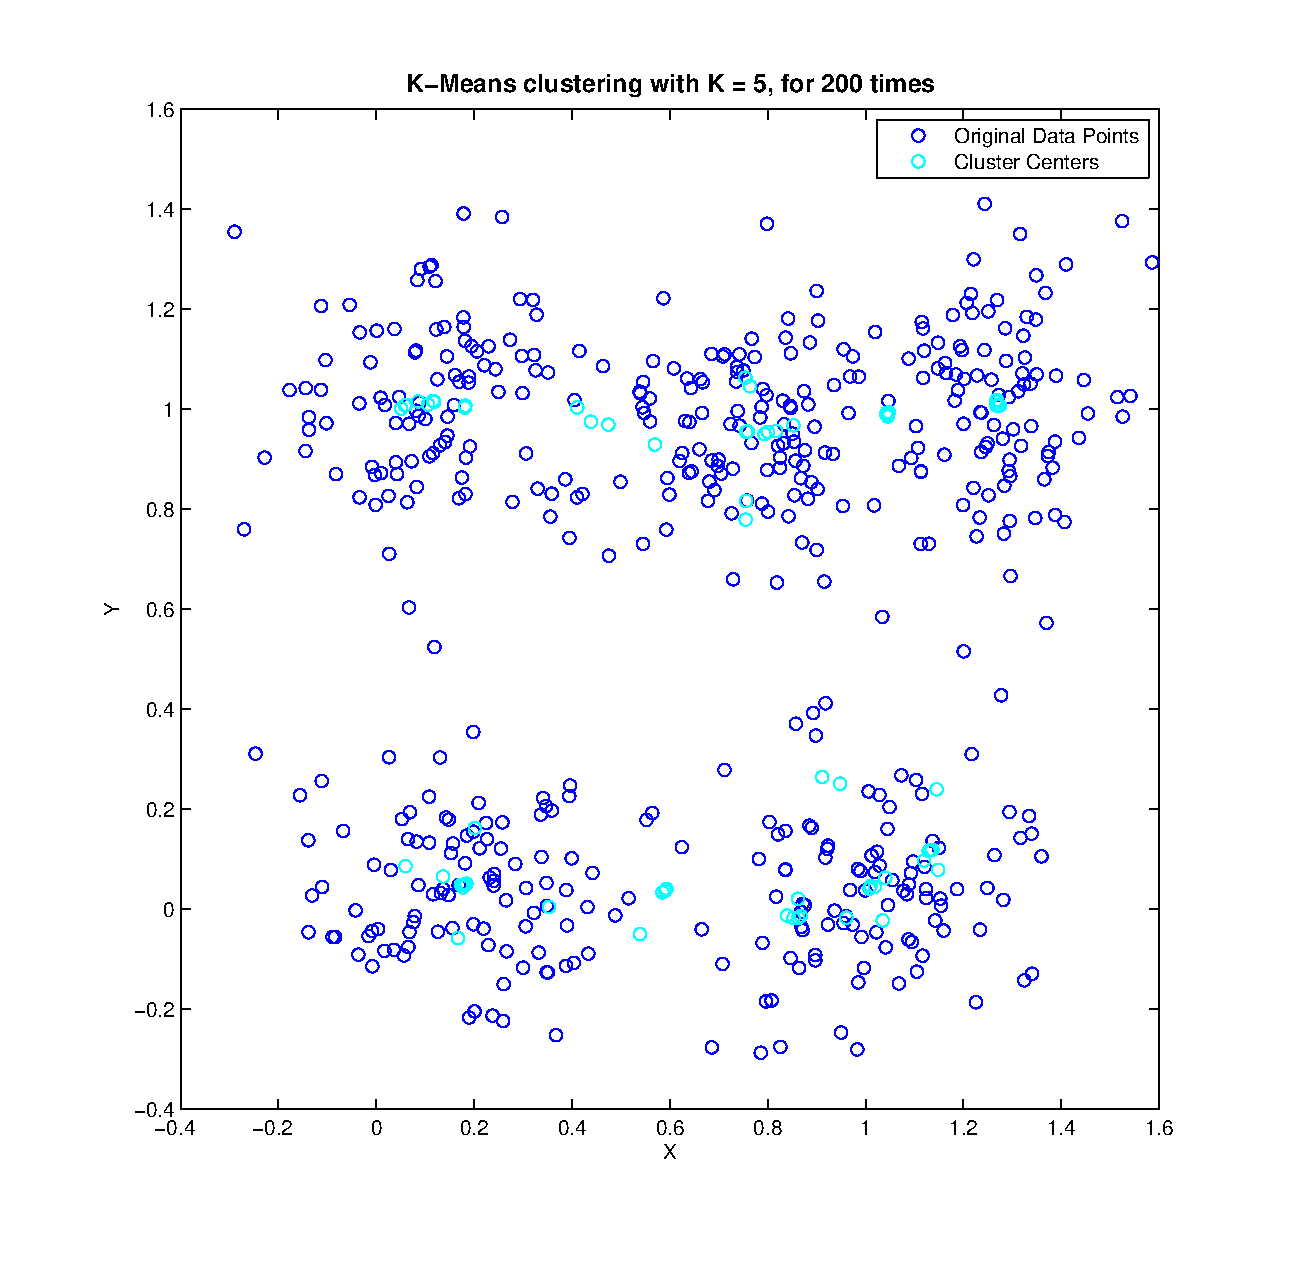
\includegraphics[width=11cm]{Fig/fig_Kmeans_with_random_initialization.eps}
 \end{center}
\caption{\small{$Kmenas$ clustering results over 200 runs.The original data points are represented in blue color and the found cluster centers are represented in cyan color}} 
\label{fig:fig_Kmeans_with_random_initialization}
\end{figure}


\section{Finding K }
Identifying how many clusters are in the data is a very challenging task. In this task, you will try out a commonly used heuristic on the provided $data2$. We will consider a variety of different k values $\left(k = 2, 3, ..., 15\right)$. For each k value, you will run your kmeans algorithm with 10 different random initializations and record the lowest within-cluster sum of squared distances obtained for that $k$ value. You will then plot them as a function of $k$.\\
a. What trend do you observe as the $k$ increase from $2$ to $15$? Do you expect this trend to be generally true for all data as we increase $k$?\\
b. A commonly used heuristic is to look for the “knee” in this curve, which is the value of k where the rate decreasing sharply reduces. Find the knees in your plot and provide an explanation to your finding. Why do we see multiple knees? what do they correspond to?\\

\begin{figure}[h]
\begin{center}
\includegraphics[width=11cm]{Fig/vote_perceptroncompareW1.png}
 \end{center}
\caption{\small{Compare the linear decision boundary of voted perceptron with averaged weights and voted perceptron}} 
\label{fig:vote_perceptroncompareW1}
\end{figure}

\section{Feature normalization}
Kmeans clustering and many other clustering methods are distance based. Distances are sensitive to feature processing such as normalization. For the given data3, please do the following.
a. Apply your implemented kmeans algorithm with k = 2 for 200 different random initializations. Record all the cluster centers that are found in these 200 runs. Plot the original data in one color and plot the cluster centers in the same figure using a different color( and shape if that helps to differentiate them).
b. Now normalize the features of the given data set. That is, first center the data to have zero mean(by subtracting the mean from the data), then rescale each feature dimension to have unit variance. Redo part a with this normalized dataset. Report the difference that you observe.
The results should be different with and without normalization. Note that this should not be taken to mean that data always need to be normalized. In some cases, the difference in scale can be truly meaningful and normalization could remove such useful information. In other cases, it is crucial to properly scale the data. The decision should be made in a case-by-case fashion.

\begin{figure}[h]
\begin{center}
\includegraphics[width=11cm]{Fig/vote_perceptroncompareW1.png}
 \end{center}
\caption{\small{Compare the linear decision boundary of voted perceptron with averaged weights and voted perceptron}} 
\label{fig:vote_perceptroncompareW1}
\end{figure}


\section{Submitted Codes}
We implemented the  code of this assignment in Matlab language. The submitted codes contains the following files:\\
 1) $regression_with_l2_regularization_closed_form_sparse_solution.m$: This file contians the code of the linear regression regularization.\\
 2) $regression_with_l2_regularization_closed_form.m$: This file contians the code of the linear regression regularization with reduced feature vector.\\
 3) $batch_perceptron.m$: This file contians the code of the preceptron\\
 4) $voted_perceptron.m$: This file contians the code of the votedPpreceptron\\
 \end{document}
\bibliographystyle{abbrv}
\footnotesize
\bibliography{nips2012}

